\documentclass[a4paper]{article}

% Use the postscript times font!
\usepackage{times}
\usepackage{soul, color}
\usepackage[hyphens]{url}
\usepackage[hidelinks]{hyperref}
\usepackage[utf8]{inputenc}
\usepackage[small]{caption}
\usepackage{amsmath}
\usepackage{amsfonts}
\usepackage{graphicx}
\usepackage{subcaption}
\usepackage{amsmath,amssymb}
\usepackage{booktabs}
\usepackage{listings}
\usepackage[a4paper, portrait, margin=1in]{geometry}
\urlstyle{same}
\usepackage{listings}
\definecolor{codegreen}{rgb}{0,0.6,0}
\definecolor{codegray}{rgb}{0.5,0.5,0.5}
\definecolor{codepurple}{rgb}{0.58,0,0.82}
\definecolor{backcolour}{rgb}{0.95,0.95,0.92}

\lstdefinestyle{mystyle}{
    backgroundcolor=\color{backcolour},   
    commentstyle=\color{codegreen},
    keywordstyle=\color{magenta},
    numberstyle=\tiny\color{codegray},
    stringstyle=\color{codepurple},
    basicstyle=\ttfamily\footnotesize,
    breakatwhitespace=false,         
    breaklines=true,                 
    captionpos=b,                    
    keepspaces=true,                 
    numbers=left,                    
    numbersep=5pt,                  
    showspaces=false,                
    showstringspaces=false,
    showtabs=false,                  
    tabsize=2
}
\lstset{style=mystyle}
\lstset{language=Python}

\usepackage{parskip}

% the following package is optional:
%\usepackage{latexsym} 

\title{
\includegraphics[scale=0.75]{images/unblogo.jpg}\\CS6735 Programming Project Report}

\makeatletter
\renewcommand\@date{{%
  \vspace{-\baselineskip}%
  \large\centering
  \begin{tabular}{@{}c@{}}
    Ethan Garnier\textsuperscript{1} \\
    \normalsize ethan.garnier78@unb.ca 
  \end{tabular}%
  \hspace{3mm}
  \begin{tabular}{@{}c@{}}
    Matthew Tidd\textsuperscript{2} \\
    \normalsize mtidd2@unb.ca
  \end{tabular}
  \hspace{3mm}
  \begin{tabular}{@{}c@{}}
    Minh Nguyen\textsuperscript{2} \\
    \normalsize mnguyen6@unb.ca
  \end{tabular}
  
  \bigskip

  \textsuperscript{1}Department of Electrical and Computer Engineering, UNB\par
  \textsuperscript{2}Department of Mechanical Engineering, UNB

  \bigskip

  \today
}}
\makeatother

\begin{document}

\maketitle

\begin{abstract}
    In the field of Artificial Intelligence and Machine Learning, it can be very easy for the complexities of learning models to be obscured away behind the black boxes that are machine learning libraries. Despite the ease of use by which these libraries present, they do not always provide a complete understanding of how the learning is taking place. To truly grasp and take advantage of machine learning, one must understand the inner workings of the learning models being applied. This assignment saw students manually implement three machine learning models to truly test their understanding of these models and how they function. These models were: Adaboost with an ID3 weak base learner, an Artificial Neural Network with back-propagation, and Naïve Bayes. In addition to manually implementing these three learning models from scratch, two machine learning problems were solved using pre-existing machine learning libraries. These problems included developing a Deep Fully-Connected Feed-Forward Artificial Neural Network, and a Convolutional Neural Network to be trained and tested on the MNIST dataset of handwritten digits.
\end{abstract}

\newpage

\section{Introduction}

\section{Adaboost with ID3 Base Learner}
The Adaptive Boosting (Adaboost) classification algorithm was successfully implemented using the Python 3 programming language. The version of Adaboost implemented used the Iterative Dichotomiser 3 (ID3) decision tree learning algorithm as a weak learner. This algorithm was trained on a dataset of English alphabet character image features and used to identify letters of the alphabet based on these features, i.e., letter recognition.

\subsection{Adaboost}
Adaboost is a boosted classifier that uses multiple weak hypotheses to build a single, strong hypothesis to be used for classification. These weak hypotheses are initially learned through a weak base learner algorithm, with the performance of these weak hypotheses dictating their weight in the final, strong hypothesis. To accomplish this, Adaboost first assigns an initial weight of $1/N$ to every training example, where $N$ is the number of training examples. Upon training of a weak hypothesis, Adaboost sums the weight of all misclassified examples against the trained weak hypothesis.  This sum, called the $error$ or $\epsilon$, is used to calculate the weight, or $\alpha$, for the given weak hypothesis according to Equation~\ref{eq:weak-h-alpha}.

\begin{equation}
    \label{eq:weak-h-alpha}
    \alpha = \frac{1}{2}\ln\left(\frac{1-\epsilon}{\epsilon}\right)
\end{equation}

This process of training weak learners and calculating the $\alpha$ of those weak learners is repeated $T$ times. On each iteration of the boosting algorithm, $t \le T$, the weights of all $N$ training examples for the next iteration, $w_{i, t+1}$, are updated according to Equation~\ref{eq:example-weight-update}.

\begin{equation}
    \label{eq:example-weight-update}
    w_{i, t+1} =
    \begin{cases} 
      w_{i,t}e^{-\alpha_t} & h_t(x_i) = y_i \\
      w_{i,t}e^{\alpha_t} & h_t(x_i) \ne y_i \\
   \end{cases}
\end{equation}

Where $w_{i,t}$ is the weight of training example $i$ for the current iteration, $\alpha_t$ is the weight of the most recently learned weak hypothesis, $h_t(x_i)$ is the classification of training example $i$ using this weak hypothesis, and $y_i$ is the correct classification of example $i$. These newly calculated weights are then normalized to ensure the sum of all training example weights is one. As can be seen from Equation~\ref{eq:example-weight-update}, the weight of incorrectly classified training examples is increased, whereas correctly classified examples have their weights decreased. The reason for this is that Adaboost wants the weak base learners to place extra emphasis on learning the incorrectly classified examples to produce a more accurate result in the end. Details on how this is executed lies within the chosen weak base learner algorithm. 

\subsection{ID3}
For this implementation of Adaboost, the ID3 algorithm was chosen as the weak base learner. ID3 is a greedy, recursive learning algorithm that generates binary decision trees from a given dataset, \textit{S}, where each internal node represents a feature by which \textit{S} is split, and leaf nodes represent a classification for the remaining examples in \textit{S}. The inductive bias of the ID3 algorithm is that it prefers shorter decision trees, building off the idea that a short hypothesis that fits the data well is unlikely to be a coincidence, as opposed to a larger hypothesis. This bias of the ID3 algorithm is enforced through its statistically based splitting criteria. At each internal node, the entropy of the dataset \textit{S} is calculated based on Equation~\ref{eq:entropy}.

\begin{equation}
    \label{eq:entropy}
    Entropy(S) = -\sum_{x \in X} p(x)log(p(x))
\end{equation}

Where $X$ is the set of all classifications in $S$, and $p(x)$ is the probability of a given classification in $S$. Once the entropy for $S$ is calculated, every attribute value for every attribute in $S$ is examined as a potential split attribute value. This is done by calculating the information gain of splitting $S$ based on that attribute value according to Equation~\ref{eq:info-gain}.

\begin{equation}
    \label{eq:info-gain}
    Gain(S, A, V) = Entropy(S) - \left(\frac{|S_{\le V}|}{|S|}\times Entropy(S_{\le V}) + \frac{|S_{> V}|}{|S|}\times Entropy(S_{> V}) \right)
\end{equation}

Where $S_{\le V}$ is the subset of training examples in $S$ whose value for attribute $A$ is less than or equal to $V$, and $S_{> V}$ is the subset of training examples in $S$ whose value for attribute $A$ is greater than $V$. The largest information gain calculated for the current internal node determines the feature and feature value by which the data will be split going to the next level of the decision tree. The fact that there are only two splits for each internal node shows that this is a binary decision tree. This splitting of training examples and building of binary decision tree continues until one of the given three base cases are met:
\begin{enumerate}
    \item Base Case 1 - Every training example in \textit{S} belong to the same class. If this is the case, then return that class.

    \item Base Case 2 - There are no remaining attributes to split the data off of. If this is the case, then return the class of majority for the training examples in \textit{S}.

    \item Base Case 3 - There are no training examples in \textit{S}. If this is the case, then return the class of majority for the training examples of the parent node.
\end{enumerate}
Base case 3 is especially important, as it is this which provides the ID3 algorithm with its generalizing power. A slight change to the ID3 algorithm was made in this implementation to account for it being used as a weak base learner in Adaboost. As previously mentioned, Adaboost will update the weights of each training example over its iterations to favor the incorrectly classified examples. The weak base learner, ID3 in this case, must therefore take these weights into account to try extra hard to correctly learn these incorrectly classified examples. This was accomplished by modifying Equation~\ref{eq:info-gain} to account for the total weight of the example subsets. This can be seen in Equation~\ref{eq:weighted-info-gain}.

\begin{equation}
    \label{eq:weighted-info-gain}
    Gain(S, A, V) = Entropy(S) - \left(\frac{\sum_{e \in S_{\le V}}w_e}{|S|}\times Entropy(S_{\le V}) + \frac{\sum_{e \in S_{> V}}w_e}{|S|}\times Entropy(S_{> V}) \right)
\end{equation}

\subsection{Predicting with Adaboost}
Once the $T$ weak hypotheses have been trained and each has their own associated weight $\alpha_t$, it is time to begin classifying test data. For each testing example $x_i$, $T$ classifications are acquired by classifying that example with each of the trained weak hypothesis. For each unique classification of $x_i$, the weights, or $\alpha_t$, of all base hypotheses that gave that classification are summed and this sum represents the weight of this classification for $x_i$. The classification with the largest weight becomes the final, or returned classification for testing example $x_i$. This process is repeated for all testing examples.

\subsection{Implementation Details}
This section will outline all details related to this implementation of Adaboost and the ID3 algorithm.

\subsubsection{Development Platform and Libraries}
As was previously mentioned, all code written to implement the Adaboost and ID3 algorithms was written in Python 3. This code was written to run on a Windows operation system, but will run on any system that can run the Python programming language. All development was conducted through the Visual Studios Code text editor, and code versioning was controlled through Git to a remote repository hosted on GitHub. The Adaboost and ID3 algorithms were written completely from scratch using only Python's built-in functions, the \textit{Numpy} Python library for mathematical operations, and the \textit{Pandas} Python library for data manipulation and representation. The \textit{scikit-learn} maching learning Python library was used for pre-processing of training and testing data, as well as for evaluating the performance of the manually implemented algorithms. This machine learning library was not included or used in any of the Adaboost or ID3 algorithm implementations. The \textit{matplotlib} and \textit{seaborn} Python libraries were used to provide statistical data visualizations for the algorithm's results.

\subsubsection{Program Structure}
Python classes were used to structure the various components of this Adaboost implementation. These classes included: \textit{AdaBoost} (adaboost.py), \textit{ID3Classifier} (id3.py), and \textit{BinaryDecisionTree} (tree.py). By following an object oriented approach, different instances of the learning algorithms could be instantiated with different hyper-parameters and then re-used when needed. This, in addition to allowing these classes to keep track of their own internal state while training, significantly cleaned up and optimized the code. For example, the \textit{AdaBoost} class has it's own internal member variables named \textit{models} and \textit{alphas} which store the trained weak hypotheses and their corresponding weights, respectively. This means that once the \textit{AdaBoost} models have been trained, these models and their weights can easily be accessed through these member variables, vastly reducing the amount of code required to keep track of this state. In addition to this, the \textit{ID3Classifier} class contains two private static methods used to calculate the entropy and information gain throughout its training process.

\subsubsection{Data-Structures}
The Dataframe data structure, as part of the \textit{Pandas} library, is a data structure that allows for data to be represented in a two-dimensional tabular format and was used extensively throughout this project. Using Dataframes allowed for the training and testing data to easily be extracted, segmented, manipulated, and represented throughout the entire training and classification process. Although operations on Dataframes are extremely slow, they also allow for the data to be exported to a two-dimensional Numpy array, and this feature was used a lot for data manipulation and calculations. Finally, Dataframes were leveraged to store training and classification results of the Adaboost algorithm in a tabular format and to export these results to a .csv file.

A binary tree data structure was manually implemented in Python to fulfill the decision tree output of the ID3 algorithm. This binary tree implementation, named \textit{BinaryDecisionTree} in tree.py, is a recursive tree data structure that possesses four attributes: 1) a split feature index, 2) a split feature value, 3) a truth branch, 4) a false branch. The split feature index of the \textit{BinaryDecisionTree} is an integer value that represents the feature this node splits on in the training data. Instead of storing the name of the feature as a string, the index of the feature in the list of feature names is stored. This is done to improve performance. The split feature value is exactly as the name describes, it is the value of the split feature by which this node splits the data on. The truth branch is a reference to another \textit{BinaryDecisionTree} object, hence the recursive nature of the data structure. When traversing the \textit{BinaryDecisionTree}, this branch is evaluated when a provided feature value is greater than the split feature value of this node. Finally, the false branch is a reference to another \textit{BinaryDecisionTree} object that is evaluated when a provided feature value is less than or equal to the split feature value of this node. The form of the trees built by the \textit{BinaryDecisionTree} object can be seen in Figure~\ref{fig:binary-decision-tree}. 

\begin{figure}[h]
    \centering
    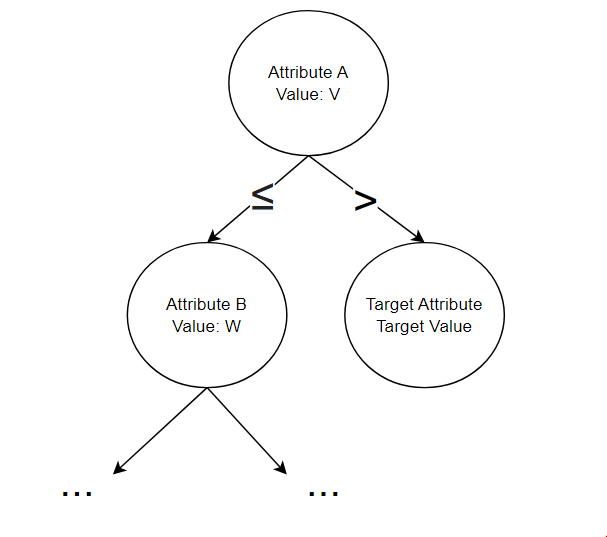
\includegraphics[scale=0.55]{images/binary-decision-tree.PNG}
    \caption{Binary decision tree created by \textit{BinaryDecisionTree} class.}
    \label{fig:binary-decision-tree}
\end{figure}

As can be seen in Figure~\ref{fig:binary-decision-tree}, leaf nodes of the tree generated by \textit{BinaryDecisionTree} have their split feature set to the target attribute of the data set, and the split feature value is the classification of the target attribute. The true and false branches are empty. As such, predictions can be made on a learned \textit{BinaryDecisionTree} for a given testing example by simply following the trees branches, checking the testing example's feature values with the split feature values at each node, until a leaf is reached where the classification for the testing example is returned.

\subsubsection{Algorithm Hyper-Parameters}
Two hyper-parameters were implemented for this Adaboost with ID3 base learner implementation. These hyper-parameters include: 1) the maximum tree depth of the learned binary decision trees, and 2) the number of weak hypotheses learned by Adaboost. 

The maximum tree depth of the learned binary decision tree is a hyper-parameter of the ID3 algorithm implementation, and it sets a limit on the maximum depth of recursion of the algorithm. This depth was monitored as a \textit{depth} parameter incremented on each recursive call. When the maximum depth was reached, the target value of majority in the current data set was returned as the leaf node. If the caller did not specify a maximum tree depth, then a tree depth of infinity was set, which essentially means the algorithm would only return a leaf node if one of its original three base cases were hit. It was experimentally determined, as can be seen in Figure~\ref{fig:depth-hyper-param}, that placing a limit on the depth of the trained binary decision tree less than the number of features in the data set actually reduces classification accuracy. For context, Figure~\ref{fig:depth-hyper-param} used a dataset with 16 features. This makes intuitive sense, as each node splits on a single feature, so there can only ever be a tree as deep as the number of features. Also, if we force a tree to terminate early, then we are forcing it to over generalize the data. Either way, this hyper-parameter remained as reducing the depth of the tree significantly improves training and classification performance. 

\begin{figure}[h]
    \centering
    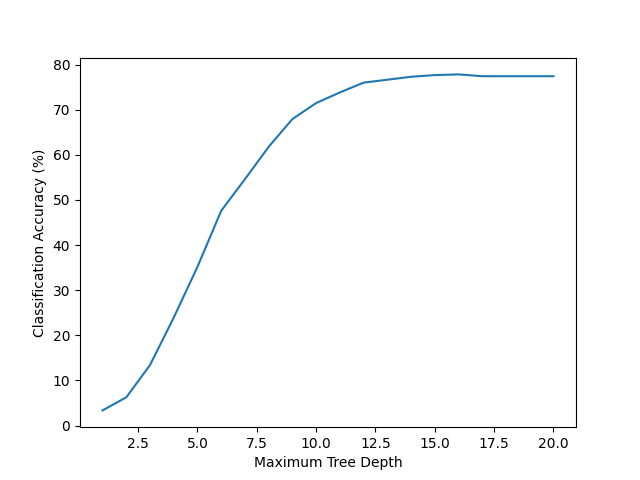
\includegraphics[scale=0.7]{images/tree-depth-plot.png}
    \caption{Accuracy of classification vs. maximum tree depth of learned binary decision tree by ID3 algorithm.}
    \label{fig:depth-hyper-param}
\end{figure}

The second hyper-parameter implemented, the number of weak hypotheses learned by the Adaboost algorithm, is a hyper-parameter of the Adaboost algorithm that controls the number of models trained by the weak base learner for a single Adaboost training session. This hyper-parameter has direct influence on the performance of the Adaboost algorithm, both from a time point-of-view and an accuracy point-of-view. The more weak hypotheses trained, the longer training will take; however, the more accurate classification can become. It was experimentally determined that 14 is the optimal number of weak hypotheses to learn as it maximizes the classification accuracy while keeping the training time as low as possible. Figure~\ref{fig:estimator-hyper-param} demonstrates how at 14 weak hypotheses, the classification accuracy of the Adaboost algorithm reaches an asymptote. Although this is only for a particular split of the dataset, it remains consistent. Figure~\ref{fig:estimator-time} shows how the time taken for training the Adaboost algorithm increases linearly with the number of weak hypotheses learned by the algorithm. As such, it is optimal to use 14 weak hypotheses to maximize classification accuracy while ensuring training time doesn't continue to increase.

\begin{figure}[h]
    \centering
    \begin{subfigure}[t]{0.48\textwidth}
        \centering
        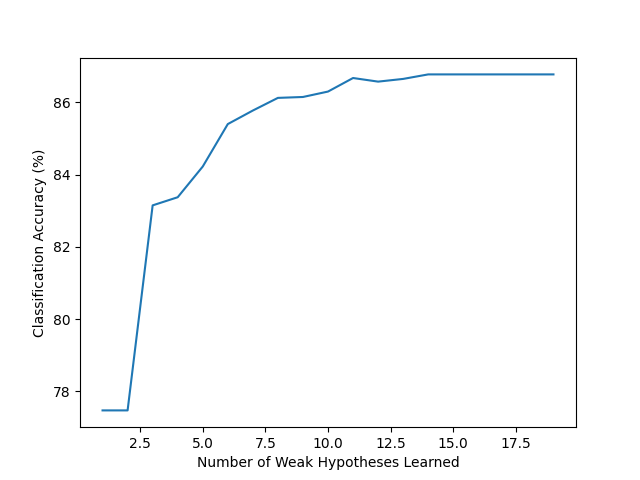
\includegraphics[width=\linewidth]{images/n-weak-hypotheses-plot.png}
        \caption{}
        \label{fig:estimator-hyper-param}
    \end{subfigure}%
    ~ 
    \begin{subfigure}[t]{0.48\textwidth}
        \centering
        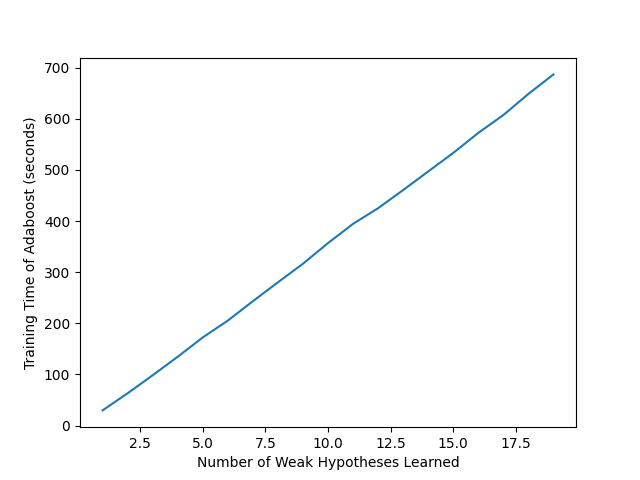
\includegraphics[width=\linewidth]{images/adaboost-training-time.png}
        \caption{}
        \label{fig:estimator-time}
    \end{subfigure}

    \caption{Performance of the number of weak hypotheses trained by Adaboost algorithm during training vs. (a) classification accuracy, and (b) time taken to train the model.}
    \label{fig:adaboost-hyper-param}
\end{figure}   

\subsection{Dataset Details}
This section will outline all details related to dataset used to train and test the Adaboost implementation. 

\subsubsection{Description of Dataset}
The dataset was taken from the UC Irvine Machine Learning Repository and has the ID 59 within this repository. The goal of the dataset is to identify each entry as a capital letter from the English alphabet based on 16 primitive numerical attributes extracted from a black-and-white image of the letter that the entry represents. The dataset contains 20 thousand entries with 17 columns for each entry, 16 columns being the previously mentioned primitive numerical attributes, and the final column being the classification of the entry, a letter in this case. These 16 primitive numerical attributes, or features in the context of machine learning, are integer values between 0 and 15 and are described as the following:
\begin{enumerate}
    \item x-box - Horizontal position of box.
    \item y-box - Vertical position of box.
    \item width - Width of box.
    \item hight - Height of box.
    \item onpix - Total number on pixels.
    \item x-bar - Mean x of on pixels in box.
    \item y-bar - Mean y of on pixels in box.
    \item x2bar - Mean x variance.
    \item y2bar - Mean y variance.
    \item xybar - Mean x y correlation.
    \item x2ybr - Mean of x * x * y.
    \item xy2br - Mean of x * y * y.
    \item x-ege - Mean edge count left to right.
    \item xegvy - Correlation of x-ege with y.
    \item y-ege - Mean edge count bottom to top.
    \item yegvx - Correlation of y-ege with x.
\end{enumerate}

The total number of classes in this dataset is 26, representing the number of capital letters in the English alphabet. The distribution of classes within the dataset is nearly uniform, as can be seen in Figure~\ref{fig:class-histogram}. As such, no re-sampling of data was needed.

\begin{figure}[h]
    \centering
    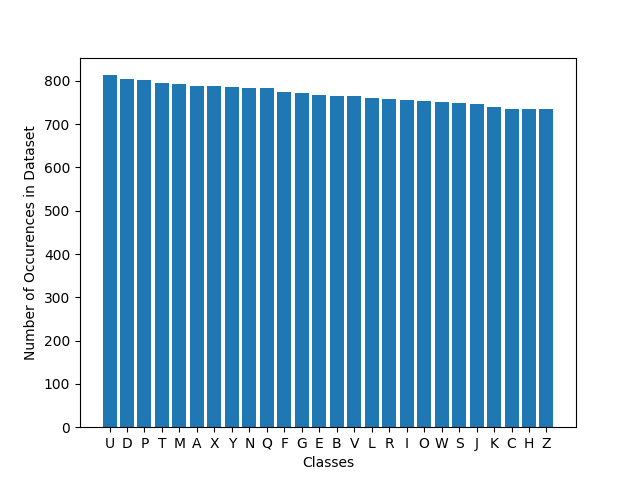
\includegraphics[scale=0.7]{images/class-distribution.png}
    \caption{Distribution of classes within the Letter Distribution dataset.}
    \label{fig:class-histogram}
\end{figure}

\subsubsection{Pre-Processing}
As previously mentioned, there are no missing values within the dataset used. As such, no pre-processing of the data to remove partial entries was required. The only pre-processing performed on the dataset was to split the data into testing and training datasets using the \textit{train\_test\_split()} function from the \textit{scikit-learn} machine learning library. A split of 80\%/20\% (16000/4000) was used for training and testing, respectively, as this was the split suggested by UC Irvine on the dataset's webpage. As such, in all results presented in the next sections, the Adaboost algorithm was trained on 16 000 randomly selected entries, and tested on the remaining 4000 entries of the dataset.

\subsection{Experimental Results}
The above discussed Adaboost algorithm with ID3 as a weak base learner implementation was tested extensively and the results of this testing can be seen in Table~\ref{tbl:adaboost-results}. As previously mentioned, these results were achieved by training the algorithm on 16 000 randomly sampled entries of the dataset, and tested on the remaining 4000 entries of the dataset. The seeds, or \textit{random\_states}, of the sampling is also reported in the table for reproducibility. The hyper-parameters were set to their previously mentioned optimal values of 16 for the maximum depth of a learned binary decision tree, and 14 for the number of weak hypotheses learned by the Adaboost algorithm.

\begin{table}[h!]
    \centering
    \begin{tabular}{||c c c c c||} 
        \hline
        Test \# & Seed & Accuracy (\%)  & Training Time (s) & Classification Time (s) \\ [0.5ex] 
        \hline\hline
        1 & 500864380 & 85.33 & 509.20 & 0.0897 \\
        \hline
        2 & 434317629 & 85.45 & 498.24 & 0.0888 \\
        \hline
        3 & 81483430 & 84.40 & 489.30 & 0.0897 \\
        \hline
        4 & 794073002 & 86.28 & 492.81 & 0.0891 \\
        \hline
        5 & 278379451 & 84.10 & 492.79 & 0.0898 \\
        \hline
        6 & 1019885152 & 84.65 & 483.37 & 0.0877 \\
        \hline
        7 & 880373647 & 85.93 & 486.33 & 0.0875 \\
        \hline
        8 & 244411609 & 85.88 & 487.19 & 0.0906 \\
        \hline
        9 & 573119018 & 83.80 & 485.92 & 0.0893 \\ 
        \hline
        10 & 496202245 & 83.03 & 487.38 & 0.0896 \\
        \hline
        11 & 136944384 & 84.18 & 500.03 & 0.0905 \\
        \hline
        12 & 131276866 & 85.80 & 486.27 & 0.0868 \\
        \hline
        13 & 276617434 & 86.70 & 482.18 & 0.0886 \\
        \hline
        14 & 817708150 & 86.60 & 478.75 & 0.0892 \\
        \hline
        15 & 44078284 & 86.68 & 505.69 & 0.0908 \\ [1ex]
        \hline
    \end{tabular}
    \caption{Results of training Adaboost implementation on 16 000 randomly sampled examples and classifying the remaining 4000 examples with maximum tree depth of 16 and 14 weak base hypotheses learned.}
    \label{tbl:adaboost-results}
\end{table}

The mean classification accuracy of the results presented in Table~\ref{tbl:adaboost-results} is 85.254\%, with the mean training and classification times being 491.03 seconds and 0.08918 seconds, respectively. Despite not achieving 100\% accuracy, the Adaboost implementation is still a success in our opinion as it is a completely from scratch implementation. The lack of accuracy in classification may come from the weighted feature info gain calculation being employed, referenced in Equation~\ref{eq:weighted-info-gain}, to place more emphasis on previously incorrectly classified examples. As for the training time, ID3 is a greedy algorithm, as such it is expected to have a longer execution time. Much work was done in the ID3 implementation to ensure all math operations were vectorized within the Python programming language to minimize the amount of looping and memory copies required. No parallelization was employed as to not over complicate the implementation, yet the routine for determining the split feature can easily be parallelized as determining the split feature based on weighted info gain can be done independently of other features.

The confusion matrix of the test with the highest accuracy, test 13 with seed 276617434, can be seen in Figure~\ref{fig:confusion-matrix}. The confusion matrix helps highlight the number of examples that were incorrectly classified, and what those incorrect classifications were compared to the correct classifications. As such, a strong diagonal of the matrix indicates high classification accuracy, as can be seen in Figure~\ref{fig:confusion-matrix}.

\begin{figure}[h!]
    \centering
    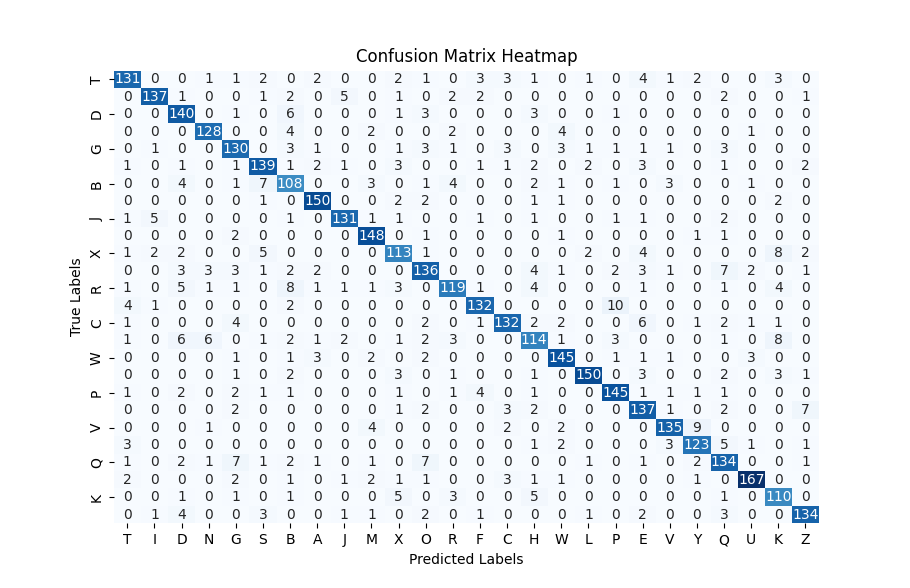
\includegraphics[scale=0.65]{images/confusion-matrix.png}
    \caption{Confusion matrix of training/classification results with seed 276617434.}
    \label{fig:confusion-matrix}
\end{figure}


\newpage

\section{ANN with Backpropagation}

An Artificial Neural Network with backpropagation was successfully implemented using the Python 3 programming language. The artificial neural network that was created featured a simplistic design, utilizing only one hidden layer while simultaneously yielding great results. This algorithm was trained on a dataset that consisted of features computed from digitized images of fine needle aspirate of breast mass, describing charactersitics of the cell nuclei present in the image. The objective was classification of cell mass as either benign or malignant.

\subsection{Artificial Neural Networks}

As mentioned, this section of the programming project saw the implementation of an artificial neural network from scratch. Artificial neural networks, or neural networks, are a machine learning technique that seek to mimic the biological neural networks found within human brains. A neural network consists of connected ``units", or nodes, that are called neurons. These neurons are designed such that they mimic the neurons found within a human brain, in the sense that they will not ``fire'', so to speak, if the input signal is not larger than a certain threshold. This thresholding is achieved through the use of an activation function, which ensures that important features that are interesting enough to be learned are actually learned by the network as they exceed the threshold. The output of a given neuron is therefore calculated by applying the activation function to the weighted sum of the inputs to that neuron. Neural networks are composed of three distinct layers, those being the input layer, the hidden layer, and the output layer. The input signal is first sent through the input layer, which takes in the data and sends it to the subsequent layers, known as the hidden layers. The hidden layers serve as an intermediary layer between the first layer and the last layer, the output layer. It is within these hidden layers that the input becomes further and further abstracted, and a new representation is learned that extracts the hidden relationship between the input features. 


For this assignment, as mentioned, a neural network was created with three layers: one input, one hidden, and one output. Justification for the choice of this structure can be found within Section \ref{ANNhyperparameterselection}. As such, the general structure of the neural network implemented is given by Figure \ref{fig:annstructure}:

\begin{figure}[h]
    \centering
    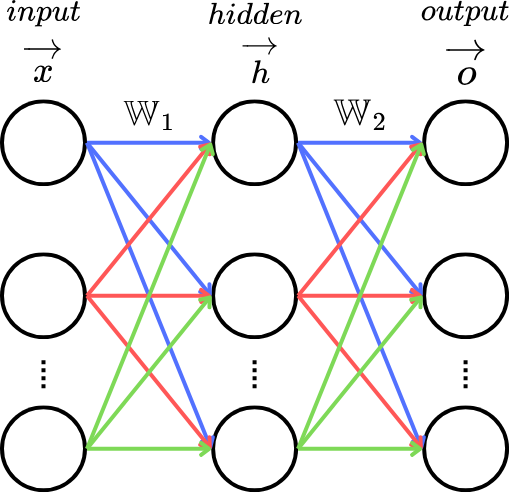
\includegraphics[scale = 0.5]{images/annstructure.png}
    \caption{Structure of the ANN that was developed.}
    \label{fig:annstructure}
\end{figure}

Where a vector of inputs $\overrightarrow{x}$ is fed into the first layer of the network, and this vector is then multiplied by the matrix of weights for the connections between the input layer and the hidden layer, $\mathbb W_1$. There is also a bias that gets added to this weighted summation, denoted by $\overrightarrow{b_1}$. This process results in what is known as the net, which is the weighted summation that is fed into the activation function of the first hidden layer. This is given by Equation \ref{eq:net1} below:

\begin{equation}
    \label{eq:net1}
    \overrightarrow{net_{1}} = \mathbb W_{1} \times \overrightarrow{x} + \overrightarrow{b_1}
\end{equation}

Following the determination of $\overrightarrow{net_{1}}$, this value is then fed into the hidden layer and the activation function is applied, which is given below by Equation \ref{eq:h1}:

\begin{equation}
    \label{eq:h1}
    \overrightarrow{h} = \sigma(\overrightarrow{net_{1}})
\end{equation}

Equation \ref{eq:h1} yields the output from the hidden layer, which is then multiplied by the weights between the hidden and output layer and added to another bias vector to get another net, shown below as:

\begin{equation}
    \label{eq:net2}
    \overrightarrow{net_{2}} = \mathbb W_{2} \times \overrightarrow{h} + \overrightarrow{b_2}
\end{equation}

Finally, the output of the network is computed by applying the activation function to $\overrightarrow{net_{2}}$, as given by:

\begin{equation}
    \label{eq:o1}
    \overrightarrow{o} = \sigma(\overrightarrow{net_{2}}) 
\end{equation}

Neural networks learn by continually updating their weights through a process known as backpropagation, which involves taking the gradient of the difference between your target value and output value, with respect to each individual weight matrix $\mathbb W_{i}$. To update the weights, we want to learn $\mathbb W$'s that minimize the square error function, given by:

\begin{equation}
    \label{eq:squarederrorfunction}
    E[\mathbb W] = \frac{1}{2} \sum_{d \in D}(t_d - o_d)^2
\end{equation}

Where $d$ represents an example from the dataset $D$, $t_d$ is the target label for that example, and $o_d$ is the output of the network. By calculating the gradient of this error function, we get:

\begin{equation}
    \label{eq:sqegradient}
    \nabla{E[\mathbb W]} = \left[ \frac{\partial{E}}{\partial{\mathbb W_o}}, \frac{\partial{E}}{\partial{\mathbb W_1}}, \ldots, \frac{\partial{E}}{\partial{\mathbb W_n}} \right]
\end{equation}

To train the network, we must update the weights according to the following equation:

\begin{equation}
    \label{eq:trainW}
    \mathbb W_i = \mathbb W_i + \Delta{\mathbb W_i}
\end{equation}

Where the incremental change in weight, $\Delta{\mathbb W_i}$, is given by the following equation:

\begin{equation}
    \label{eq:deltaW}
    \Delta{\mathbb W_i} = -\eta \frac{\partial{E}}{\partial{\mathbb W_i}}
\end{equation}

Where $\eta$ is the \textit{learning rate}, which determines the size of the step to be taken during the gradient descent algorithm. The value of $\frac{\partial{E}}{\partial{\mathbb W_i}}$ is given by the following derivation:

\begin{gather}
    \begin{aligned}
        \frac{\partial{E}}{\partial{\mathbb W_i}} &= \frac{\partial}{\partial{\mathbb W_i}} \frac{1}{2} \sum_{d \in D}(t_d - o_d)^2 \\
        &= \frac{1}{2}\sum_{d \in D}\frac{\partial}{\partial{\mathbb W_i}}(t_d - o_d)^2 \\
        &= \sum_{d \in D}(t_d - o_d)\frac{\partial}{\partial{\mathbb W_i}}(t_d - o_d) \\
        &= \sum_{d \in D}(t_d - o_d)\left[-\frac{\partial{o_d}}{\partial{\mathbb W_i}}\right] \\
        &= -\sum_{d \in D}(t_d - o_d)\left[\frac{\partial{o_d}}{\partial{\mathbb W_i}}\right] \\
        \therefore \frac{\partial{E}}{\partial{\mathbb W_i}} &= \sum_{d \in D}(o_d - t_d)\left[\frac{\partial{o_d}}{\partial{\mathbb W_i}}\right]
    \end{aligned}
\end{gather}

Where the value of $\sum_{d \in D}(o_d - t_d)$ is equal to the gradient of the error with respect to the output value $o_d$, as evidenced by Equation \ref{eq:delEdelod}:

\begin{gather}
    \begin{aligned}
        \label{eq:delEdelod}
        \frac{\partial{E}}{\partial{o_d}} &= \sum_{d \in D}(o_d - t_d) \\
        \frac{\partial}{\partial{o_d}}\frac{1}{2}\sum_{d \in D}(t_d - o_d)^2 &= \sum_{d \in D}(o_d - t_d) \\
        \sum_{d \in D}(t_d - o_d)(-1) &= \sum_{d \in D}(o_d - t_d)\\
        \therefore \sum_{d \in D}(o_d - t_d) &= \sum_{d \in D}(o_d - t_d)
    \end{aligned}
\end{gather}

From this, it can be gathered that to update any $\mathbb W_i$, we can use the following equation:

\begin{equation}
    \label{eq:keyweightupdating}
    \mathbb W_i = \mathbb W_i - \eta \left[ \frac{\partial{E}}{\partial{o_d}}\times\frac{\partial{o_d}}{\partial{\mathbb W_i}} \right]
\end{equation}

Meaning that for each layer, the value of $\frac{\partial{o_d}}{\partial{\mathbb W_i}}$ needs to be determined such that each weight matrix can be updated. For the second weight matrix, this derivation is given by Equation \ref{eq:w2update}. The $d$ subscript is dropped as it was assumed that stochastic gradient descent would be employed, which obviously is performed on each training example $d \in D$.

\begin{gather}
    \begin{aligned}
        \label{eq:w2update}
        \frac{\partial{o}}{\partial{\mathbb W_2}} &= \frac{\partial}{\partial{\mathbb W_2}}\sigma(\overrightarrow{net_2}) \\
        &= \frac{\partial}{\partial{\mathbb W_2}}\sigma(\mathbb W_2 \sigma(\mathbb W_1 \overrightarrow{x})) \\
        \therefore \frac{\partial{o}}{\partial{\mathbb W_2}} &= \sigma'(\overrightarrow{net_2})h
    \end{aligned}
\end{gather}

Similarly, this process was repeated for $\mathbb W_1$:

\begin{gather}
    \begin{aligned}
        \label{eq:w1update}
        \frac{\partial{o}}{\partial{\mathbb W_1}} &= \frac{\partial}{\partial{\mathbb W_1}}\sigma(\overrightarrow{net_2}) \\
        &= \frac{\partial}{\partial{\mathbb W_1}}\sigma(\mathbb W_2 \sigma(\mathbb W_1 \overrightarrow{x})) \\
        &= \sigma'(\overrightarrow{net_2})\frac{d}{d{\mathbb W_1}}\left[ \mathbb W_2 \sigma(\mathbb W_1 \overrightarrow{x}) \right]\\
        \therefore \frac{\partial{o}}{\partial{\mathbb W_1}} &= \sigma'(\overrightarrow{net_2})\mathbb W_2 \sigma'(\overrightarrow{net_1})\overrightarrow{x}
    \end{aligned}
\end{gather}

The question therefore arose, how will the bias be updated? It was determined that the bias would be updating using a similar approach to Equation \ref{eq:trainW}, where the bias updating equation is given below as:

\begin{equation}
    \label{eq:trainBias}
    b_i = b_i - \eta \frac{\partial{E}}{\partial{b_i}}
\end{equation}

Where the partial derivative of error with respect to the bias value $b_i$ is given by:

\begin{gather}
    \begin{aligned}
        \label{eq:biasderivation}
        \frac{\partial{E}}{\partial{b_i}} &= \frac{\partial}{\partial{b_i}}\left[ \frac{1}{2} \sum_{d \in D}(t_d - o_d)^2 \right] \\
        &= \frac{1}{2}\sum_{d \in D} \frac{\partial}{\partial{b_i}}(t_d - o_d)^2 \\
        &= \sum_{d \in D}\frac{\partial}{\partial{b_i}}(t_d - o_d) \\
        &= \sum_{d \in D}(t_d - o_d)\frac{\partial}{\partial{b_i}}(-o_d) \\
        \therefore \frac{\partial{E}}{\partial{b_i}} &= \sum_{d \in D}(o_d - t_d)\frac{\partial{o_d}}{\partial{b_i}}
    \end{aligned}
\end{gather}

Where the value of $\sum_{d \in D}$ is known by Equation \ref{eq:delEdelod}, which implies that the partial derivative of error with respect to bias is equal to:

\begin{equation}
    \label{eq:delEdelbias}
    \frac{\partial{E}}{\partial{b_i}} = \frac{\partial{E}}{\partial{o_d}} \times \frac{\partial{o_d}}{\partial{b_i}}
\end{equation}

The expanded equation of the output from our network, with biases included, is given below within Equation \ref{eq:outputwithbias}. The biases were initially neglected when determining the weight matrices as they are not functions of the weight, and therefore were dropped when the partial derivative of error with respect to the weight matrices was performed. 

\begin{equation}
    \label{eq:outputwithbias}
    \overrightarrow{o} = \sigma(\mathbb W_2 \sigma(\mathbb W_1 \overrightarrow{x} + \overrightarrow{b_1}) + \overrightarrow{b_2})
\end{equation}

Therefore, we just need to determine the value of $\frac{\partial{o_d}}{\partial{b_i}}$ for each layer. For $b_2$, this is done as follows:

\begin{gather}
    \begin{aligned}
        \frac{\partial{o_d}}{\partial{b_2}} &= \frac{\partial}{\partial{b_2}}\sigma(\overrightarrow{net_2} + \overrightarrow{b_2}) \\
        \frac{\partial{o_d}}{\partial{b_2}} &=\sigma'(\overrightarrow{net_2})
    \end{aligned}
\end{gather}

For $b_1$, this is done as follows:

\begin{gather}
    \begin{aligned}
        \frac{\partial{o_d}}{\partial{b_1}} &= \frac{\partial}{\partial{b_1}} \sigma(\mathbb W_2 \sigma(\mathbb W_1 \overrightarrow{x} + \overrightarrow{b_1}) + \overrightarrow{b_2})\\
        \frac{\partial{o_d}}{\partial{b_1}} &= \sigma'(\overrightarrow{net_2})\mathbb W_2 \sigma'(\overrightarrow{net_1})
    \end{aligned}
\end{gather}

The general workflow for utilizing the neural network is as follows:

\begin{enumerate}
    \item A neural network object is instantiated from a class, specifying the input size, the hidden layer size, and output size.
    \item This network is then trained, using a training function that is contained within the object. This training procedure calculates a forward pass first by passing the input vector through the network, which yields an output. This output, as well as the target values from the input vector and a learning rate are passed through a backward pass, which updates the weights using the backpropagation equations determined above.
    \item Once the network has been trained, it can be tested by passing it features and labels, where it calculates the accuracy of the model based on how many it correctly classifies.
\end{enumerate}

With all of the pertinent equations for the backpropagation algorithm determined, as well as the workflow, the focus then turned towards the actual implementation of the neural network through code for performing classification on the given dataset.

\subsection{Implementation Details}

This section outlines all details related to the implementation of the neural network, including the development platform and libraries used, the programmatic structure, the data structures used, and the choice of hyperparameters.

\subsubsection{Development Platform \& Libraries Used}

As was previously mentioned, all code written to implement the neural network with backpropagation was written in Python 3. The code was written on a Windows operating system, and was not tested on other operating systems, but it is assumed that it will run on any system that can run the Python programming language. The development of this algorithm was done using Microsoft's Visual Studio Code. The environment was configured to run Jupyter Notebook .ipynb files, which due to their ability to run code one cell at a time, are favoured for machine learning development. The Python 3 kernel that was utilized within this .ipynb environment was Python 3.12.5. Code versioning was controlled through Git utilizing a remote repository hosted on GitHub. The neural network itself, as well as the backpropagation algorithm, were written completely from scratch using Python's built-in functionalities as well as the \textit{Numpy} Python library for mathematical operations. The \textit{Pandas} Python library was utilized for data manipulation and exploratory analysis, and the \textit{scikit-learn} machine learning Python library was used to apply pre-processing to the data, as well as performing the train/test split. It must be noted that this machine learning library was not used for anything other than splitting data and applying standardization. It was not incorporated within the actual neural network class, and did not contribute to the development of the neural network other than being a tool for data separation and scaling. The \textit{matplotlib} and \textit{seaborn} Python libraries were utilized for visualization of both training and testing results, and the \textit{csv} python package was used to save initial weights when a good run occurred and load them to initialize the network. Finally the UC Irvine Machine Learning Python package \textit{ucimlrepo} was used to fetch the dataset, which was hosted on their website. 

\subsubsection{Program Structure}

The neural network code was implemented using a .ipynb file within VS Code, as mentioned previously. This meant that the code could be partitioned into sections, and each section must be run sequentially for the code to function. The sections are as follows:

\begin{enumerate}
    \item Importing Packages
    \item Loading the Dataset
    \item Examining the Dataset Properties
    \item Dataset Pre-Processing
    \item Function Definition
    \item Training \& Testing the Model
\end{enumerate}

The general workflow of the program is as follows. Firstly, the relevant packages necessary to utilize the code are imported. Following this, the dataset is fetched from the UC Irvine Machine Learning repository. An exploratory analysis is performed on the data, which gets the total number of instances, the number of features, the number of unique target variables, and the names of each feature. Following this, the dataset is pre-processed, where it is examined for null values and standardized, and the labels are binary encoded from categorical values. Several functions are defined, as well as the main neural network class. A sigmoid function and its derivative were defined, as well as a ReLu function and its derivative. A binary cross entropy loss function was defined since the classification task is binary in nature. Following this, the neural network class was defined.

As previously mentioned, an object-oriented approach was implemented for the neural network architecture. This allowed training, testing, and instantiating the network to be done utilizing functions inherent to the class. The class contains a constructor that takes the number of input neurons, the number of hidden neurons, and the expected output size. Within this constructor, weights are randomly initialized from a normal distribution. A feedforward function was defined that takes in the vector of inputs, and ensures that this vector is a column vector. Following this, the net and activated net are calculated for each layer, and the output is returned. A backpropagation function was defined that performs the backpropagation procedure for every weight and bias value, in accordance with the equations derived in Section \ref{ANNtheory}.

The neural network class also contains training and testing functions. The training function takes in the training x and y values, as well as the validation x and y values, a number of epochs, and a learning rate. This training function utilizes every feature and computes the forward pass and back propagates for every example, for every epoch. In this regard, the training process utilizes stochastic gradient descent. The average binary cross entropy across all training examples per epoch is calculated as a loss metric, and a similar process occurs for validation data. This function returns the training loss history and the validation loss history. 

The testing function effectively computes the forward pass, and extracts a class value from the sigmoid layer result, and if this predicted value is the same as the target, it increments the number of correct predictions. Accuracy is calculated as the number of correct predictions divided by the number of testing values examined. With the pertinent functions defined, a network is instantiated from the class, and it is trained using the training and validation data. Following this, the training and validation loss is plotted with respect to epochs, and the network is tested. A confusion matrix is generated to visualize the efficacy of the model. This entire process can be run by selecting ``run all" within the .ipynb file.


\subsubsection{Data Structures Used}

When the data is initially fetched from the remote repo, it is imported as a special data structure called \textit{ucimlrepo.dotdict.dotdict}. This data type seems to be a dictionary of Pandas data frames because the feature and target values are stored within Pandas data frames. As mentioned previously, Pandas data frames were used extensively throughout this project due to their ease of manipulation and representation. This data frame structure allowed for exploratory analysis to be performed on the feature data, and the dataset could be examined in terms of how many instances there were, the number of features, the number of unique target variables, and the name of the features. A Pandas data frame also allows for using the \textit{.head()} handle to examine the first five rows of data, which allowed for quick visualization as the data was manipulated.

Numpy arrays were utilized within the forward and backward pass operations due to their ease of mathematical computation and speed of computation compared to Pandas data frames. These arrays were also utilized to store the weights, biases, and activated nets of the network due to the mathematical operations to be performed using them. Data was fed into the network by extracting each row of the data frame and converting it to a Numpy column vector. Finally, lists were utilized to store the training and validation loss history, as well as the correct predictions and target values used in formulating the confusion matrix.

\subsubsection{Hyperparameter Selection}\label{ANNhyperparameterselection}

As was mentioned, the network designed had three layers: an input layer, a singular hidden layer, and an output layer. It was decided that the network would have one hidden layer for ease of formulation, and because of the simplicity of the binary classification task to be performed. Having one hidden layer made deriving the backpropagation equations simpler, as only four equations had to be determined: two for weights and two for biases. The network was able to extract the required relationships for correctly classifying a cell mass as benign of malignant at just one layer. As such, it was deemed that a single hidden layer was enough. It was decided that the activation function to be used within the hidden layer was to be a ReLu function, and the activation function to be used at the output was a sigmoid. The ReLu function was chosen to potentially combat any problems related to updating the weights, and the probabilistic sigmoid function was chosen because the classification task to be performed was binary, and the sigmoid function is capable of outputting within a range between 0 and 1. 

Therefore, the hyperparameters explored were the number of epochs, the learning rate, and the number of neurons within the hidden layer. 10 hyperparameter combinations were explored, and the average accuracy after 5 runs was recorded for each combination. This process was done to determine which hyperparameter combination had a higher accuracy on average, as that would lead to the best model performance. All of these tests were performed by randomly sampling the weights from a normal distribution, which had the downside of a fluctuating accuracy that could perform very poorly if the initial weights used for gradient descent were poor. This process then allowed for determining a good set of initial weights and biases, which were then flattened and stored into a CSV that is now loaded every time the model is ran. This hyperparameter analysis was therefore utilized to determine the best combination of hyperparameters and the best initial weights to be used. Weights and biases are not hyperparameters, but the combination of hyperparameters that produced the best accuracy was then examined further to determine the best initial weights. The results of this hyperparameter analysis are shown below within Table \ref{tbl:hyperparametertesting}.
\newpage

\begin{table}[h!]
    \centering
    \begin{tabular}{||c c c c c||} 
        \hline
        Test \# & Epochs & $\eta$ & \# Hidden Neurons & Average Accuracy (\%) \\ [0.5ex] 
        \hline\hline
        1 & 1000 & 0.0001 & 30 & 91.99 \\
        \hline
        2 & 1000 & 0.00025 & 30 & 94.65 \\
        \hline
        3 & 1000 & 0.0005 & 30 & 93.72 \\
        \hline
        4 & 1000 & 0.001 & 30 & 96.28 \\
        \hline
        5 & 1500 & 0.0001 & 30 & 93.67 \\
        \hline
        6 & 1500 & 0.00025 & 30 & 96.05 \\
        \hline
        7 & 1500 & 0.0005 & 30 & 95.81 \\
        \hline
        8 & 1500 & 0.001 & 30 & 95.35 \\
        \hline
        9 & 1000 & 0.001 & 15 & 96.28 \\ 
        \hline
        10 & 1000 & 0.001 & 45 & 94.88 \\
        \hline
    \end{tabular}
    \caption{Average accuracy after 5 trials for each hyperparameter combination explored.}
    \label{tbl:hyperparametertesting}
\end{table}

The highest average accuracy after 5 runs was exhibited by Test 4, which was trained at 1000 epochs, a learning rate of 0.001, and had 30 hidden nodes. It was generally observed that as the number of hidden nodes increased, the accuracy fell. Lower numbers of hidden nodes had sporadic accuracy that varied greatly, with outliers that were omitted from the average accuracy calculation. This combination of hyperparameters was capable of producing an accuracy that was as high as 98.837\%, the highest accuracy that was exhibited. The initial weights and biases from this 98.837\% test run were saved as a CSV, and the neural network class was updated to include an option to utilize the saved weights. If the user does not want to load the weights, the weights and biases are randomly sampled.

\subsection{Dataset Details}

The dataset used was from the UC-Irvine Machine Learning Repository and was donated by the University of Wisconsin-Madison in 1995. It is considered a multivariate dataset, consisting of several breast mass features that were computed from digitized images of fine needle aspirate. These features describe the characteristics of the cell nuclei present within a given image. 10 real-valued features are of importance for this dataset, those being:

\begin{enumerate}
    \item radius (mean distances from the center to points on the perimeter)
    \item texture (standard deviation of gray-scale values)
    \item perimeter of the cell mass
    \item area of the cell mass
    \item smoothness (local variation in radius lengths)
    \item compactness (measured by dividing the squared perimeter by the area, and subtracting 1)
    \item concavity (severity of concave portions of the contour)
    \item concave points (number of concave portions of the contour)
    \item symmetry of the cell mass
    \item fractal dimension (statistical metric for complexity, measured using the ``coastline approximation" - 1)
\end{enumerate}

For each of these real-valued features, there are 3 versions. These versions represent the mean, standard deviation, and worst-case value of each feature. In total, there are 30 features in this dataset. The target variable within this dataset is a diagnosis, either benign or malignant, which are represented categorically as either a B or an M, respectively. There were 569 examples within this dataset. The dataset was loaded using the UCI-ML \textit{fetchrepo} command and was subsequently ready for processing. 

\subsection{Data Pre-processing}

As mentioned, the dataset was loaded using the \textit{fetch\_ucirepo} command from the UCI-ML Python package. This command fetched the dataset from the UCI website, utilizing its intrinsic dataset ID, which was 17. This data was saved into a variable called \textit{breast}, as a unique class from the UCI-ML package, called \textit{ucimlrepo.dotdict.dotdict}, which is seemingly a dictionary-based class. This data was then split into features and target labels, by calling either \textit{.data.features} or \textit{.data.targets}, respectively. The feature values were saved into a Pandas data frame called \textit{breast\_x}, whereas the target values were saved into a Pandas data frame called \textit{breast\_y}. Following the importing and analysis of the Wisconsin Breast Cancer dataset, there arose a need to pre-process the data, as is the case with most machine learning applications. The pre-processing that was performed was an inquiry into the existence of null values, standardization of the values such that their values fell within a common range, and the categorical labels were encoded into binary 0 or 1, where 0 represents benign, and 1 represents malignant. 

Null values were examined using the \textit{.isnull()} handle for Pandas data frames, combined with the \textit{.values.any()} handle from Python. This returned either True for null values, or False if no null values existed. If any null values were found within the dataset, the \textit{.dropna()} handle for Pandas data frames was used to remove all null values. This process was repeated for both the features and target values. Following this, the feature value was standardized. This was performed as the features of the input dataset had vast differences between their ranges, since different units were used for different features, as some measurements pertained to distances whereas some measurements pertained to areas or dimensionless concepts such as texture. The \textit{StandardScaler()} function from \textit{sklearn} was utilized to standardize the feature data. Finally, the categorical variables were encoded by indexing the ``Diagnosis" column of the target data frame, and mapping the value to 1 if the row value was ``M", and 0 if else. This effectively encoded the categorical data into a binary encoding suitable for use in a neural network. Following this, the dataset was split into 70\% training and 30\% testing/validation, which was then split using a 50-50 split. The entirety of this process can be seen within Appendix \hl{INSERT APPENDIX REF}.

\subsection{Experimental Results}

After detailing the theoretical background for the ANN structure, the libraries, platform, and data structures used, as well as the process of determining hyperparameters and analyzing the data set, it was thus time to test the dataset. Utilizing the hyperparameters and initialized weights determined in Section \ref{ANNhyperparameterselection}, the model was trained on the training data and the loss for both training and validation was visualized. Following this, the model was tested against the test dataset and a confusion matrix was generated to visualize its efficacy. To evaluate the model, the code was ran 10 times and the average accuracy was calculated. This meant that 10 models were generated with initialized weights, utilizing the same hyperparameters, and tested against a test set that was unique to that run. The average accuracy of the model after experimental evaluation was 95.56\%, with the highest measured accuracy being 98.837\%, and the lowest accuracy being 91.86\%. The training results and testing confusion matrix of the highest run are shown within Figures \ref{fig:anntrain} and \ref{fig:anncm}, respectively. 

\begin{figure}[h]
    \centering
    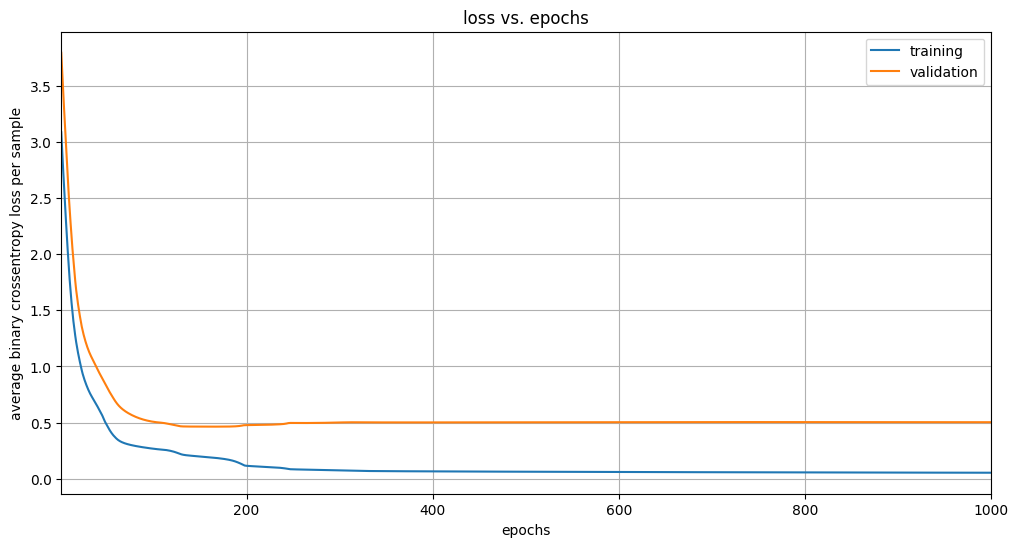
\includegraphics[width=0.9\linewidth]{images/ANNtrain.png}
    \caption{Training results of the best run for testing the ANN.}
    \label{fig:anntrain}
\end{figure}

\begin{figure}[h]
    \centering
    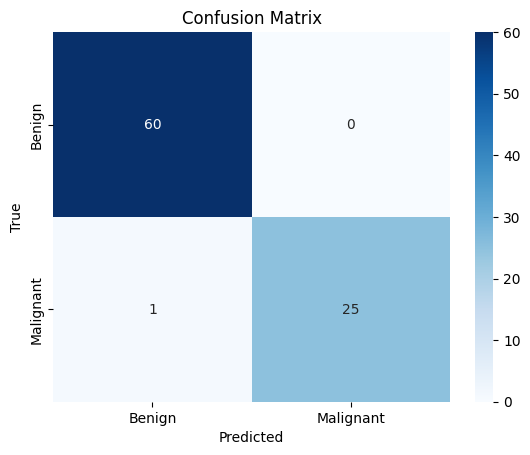
\includegraphics[width=0.8\linewidth]{images/ANNcm.png}
    \caption{Confusion matrix results of the best run for testing the ANN.}
    \label{fig:anncm}
\end{figure}
\newpage

Overall, we are satisfied with the performance of the neural network. The developers of the dataset report an average accuracy of 92.308\% utilizing a neural network for classification, and for this neural network implementation developed from scratch, we are more than happy to find that we have exceeded this value. Loading the initialized weights and biases helped tremendously in the accuracy of the model by removing the possibility of severely low weights. Before initializing the weights from a set of pre-determined weights, there were instances where the test accuracy would be exceedingly low, as low as 65\% due to poor random sampling of initial weights. This would cause the training loss to never come down and approach a value close to zero, and as such the model performed quite poorly. By initializing the weights to a good initial guess, even when the model performed poorly it only reached a low accuracy of 91.86\%, far better than 65\%. The accuracy fluctuates around $\sim$ 95\% currently, and the performance varies due to the random nature of training using backpropagation and stochastic gradient descent. Because the training data is also randomized when it is split, some training runs might see examples with easy-to-extract relationships initially, whereas others might have closely related values that are not easy to determine.

This model also has its performance capped due to only having 1 hidden layer, and might even realize higher levels of accuracy with a deeper network, but the average accuracy for this model was deemed to be sufficient for this application. As seen within Figure \ref{fig:anntrain} the model does not seem to be overfitting, as evidenced by the validation loss that steadily plateaus instead of increasing. The confusion matrix for the best test, as shown in Figure \ref{fig:anncm}, showcases that even for a partially imbalanced test set, the model is still able to realize high performances. Future work for this model could entail utilizing a deeper network, or processes such as dropout, regularization, or the use of batches.

\newpage
\section{Conclusion}

\newpage
% Bibliography/Reference Stuff
\bibliographystyle{abbrv}
\bibliography{main}

\renewcommand{\thesection}{Appendix \Alph{section}: \hspace{-4mm}}
\setcounter{section}{0} % Reset section counter

\newpage
\section{Adaboost w/ ID3 Code}

\newpage
\section{Neural Network Code}
\textbf{Importing Packages:}
\begin{lstlisting}[basicstyle= \scriptsize]
# import packages:
from ucimlrepo import fetch_ucirepo                   # used to fetch dataset
import numpy as np                                    # used for math operations
import pandas as pd                                   # used to manipulate data
from sklearn.model_selection import train_test_split  # used to split the data
from sklearn.metrics import confusion_matrix          # used to make cm
from sklearn.preprocessing import StandardScaler      # used to standardize the data
import csv                                            # used to load CSVs

import seaborn as sns                 # used for visualization of confusion matrix
import matplotlib.pyplot as plt       # used for visualization of training loss
\end{lstlisting} 

\textbf{Loading the Dataset:}
\begin{lstlisting}[basicstyle= \scriptsize]
# because the dataset is from the UCI ML repo, we can use their functions to fetch from their website:
breast_data = fetch_ucirepo(id = 17)

# can now access the data:
breast_x = breast_data.data.features    # extract the features from the dict into a pandas data frame
breast_y = breast_data.data.targets     # extract the labels from the dict into a pandas data frame
\end{lstlisting}

\textbf{Examining Dataset Properties:}
\begin{lstlisting}[basicstyle= \scriptsize]
# get the total number of instances:
print(f"there are {breast_x.shape[0]} examples in the dataset")

# get number of features:
print(f"there are {breast_x.shape[1]} distinct features to train on")

# get the number of unique target variables:
print(f"the available diagnoses are: {breast_y['Diagnosis'].unique()}")

# get the names of the features:
print(f"the available features are: \n")
for col in breast_x.columns:    # for every column in the data frame, 
    print(col)                  # print the column    
\end{lstlisting}

\textbf{Dataset Pre-Processing:}
\begin{lstlisting}[basicstyle= \scriptsize]
# check for null values in the features:
null = breast_x.isnull().values.any()   

# if any null values exist, drop them, else pass
if null == True:
    breast_x = breast_x.dropna() 
    print(f'null values removed from features')
else:
    print(f'no null values detected in features')

# check for null values in the labels, same process as above
null = breast_y.isnull().values.any()
if null == True:
    breast_y = breast_y.dropna()
    print(f'null values removed from labels')
else:
    print(f'no null values detected in labels')
    
# standardize values by defining a scaler and fitting data to scaler:
scaler = StandardScaler()
x_scaled = pd.DataFrame(scaler.fit_transform(breast_x))
print('features scaled')

# encode benign to 0, and malignant to 1
breast_y =  pd.DataFrame(breast_y['Diagnosis'].map(lambda row: 1 if row == 'M' else 0))
print('labels encoded: M = 1, B = 0')
breast_y.head()

# partition data -> want 70% train, 15% validation, 15% testing
x_train, dummy_x, y_train, dummy_y = train_test_split(x_scaled, breast_y, train_size = 0.7, test_size = 0.3)
x_val, x_test, y_val, y_test = train_test_split(dummy_x, dummy_y, train_size = 0.5, test_size = 0.5)

print(f"training data has form: {x_train.shape}, labels are: {y_train.shape}")
print(f"validation data has form: {x_val.shape}, labels are: {y_val.shape}")
print(f"test data has form: {x_test.shape}, labels are: {y_test.shape}")
\end{lstlisting}

\textbf{Function Definition:}
\begin{lstlisting}[basicstyle= \scriptsize]
# define useful functions:

# logistic sigmoid function
def sigmoid(x):
    return 1 / (1 + np.exp(-x))

# derivative of the sigmoid function
def sigmoid_derivative(x):
    return sigmoid(x) * (1 - sigmoid(x))

# rectified linear unit (basically a straight line)
def relu(x):
    return np.maximum(0, x)

# derivative function of relu (accepts np.arrays)
def relu_derivative(x):
    return (x > 0).astype(float)

# binary cross entropy -> for binary classification between 0 & 1
def binary_crossentropy_loss(target, output):
    output = np.clip(output, 1e-10, 1 - 1e-10)                              # clip to prevent log 0
    loss = - (target * np.log(output) + (1 - target) * np.log(1 - output))  # BCE formula
    return loss    
\end{lstlisting}
\newpage
\textbf{Neural Network Class Definition:}

\begin{lstlisting}[basicstyle= \scriptsize]
# create neural network class:
"""
this class accepts:

input_size: number of input neurons
hidden_size: number of hidden neurons
output_size: expected number of output neurons
load: whether or not to load initialized weights

"""
class NeuralNetwork:
    # constructor:
    def __init__(self, input_size, hidden_size, output_size, load):
        # assign function inputs as instance variables:
        self.input_size = input_size        # assign input neurons
        self.hidden_size = hidden_size      # assign hidden neurons
        self.output_size = output_size      # assign output neurons

        # if the user wants to load the pre-initialized weights and biases:
        if load == True:
            # open the CSV and read it:
            with open('initial_weights.csv', 'r') as f:
                reader = csv.reader(f)

                # for every value in each row, return as float to np.array:
                w1_flat = np.array([float(val) for val in next(reader)])
                b1_flat = np.array([float(val) for val in next(reader)])
                w2_flat = np.array([float(val) for val in next(reader)])
                b2_flat = np.array([float(val) for val in next(reader)])

                # ensure that weights are in the correct dimensions:
                self.w1 = w1_flat.reshape(hidden_size, input_size)
                self.b1 = b1_flat.reshape(hidden_size, 1)
                self.w2 = w2_flat.reshape(output_size, hidden_size)
                self.b2 = b2_flat.reshape(output_size, 1)

                # print to user that it was a success:
                print('weights loaded')
                print("w1 shape:", self.w1.shape, 'w1 type:', type(self.w1))
                print("b1 shape:", self.b1.shape, 'b1 type:', type(self.b1))
                print("w2 shape:", self.w2.shape, 'w2 type:', type(self.w2))
                print("b2 shape:", self.b2.shape, 'b2 type:', type(self.b2))

        # if not, randomly initialize weights and biases for the layers:
        else:

            # from input to hidden:
            self.w1 = np.random.randn(hidden_size, input_size)
            self.b1 = np.random.randn(hidden_size, 1)

            # from hidden to output:
            self.w2 = np.random.randn(output_size, hidden_size)
            self.b2 = np.random.randn(output_size, 1)

            # print to user that it was a success:
            print('weights randomly initialized')
            print("w1 shape:", self.w1.shape, 'w1 type:', type(self.w1))
            print("b1 shape:", self.b1.shape, 'b1 type:', type(self.b1))
            print("w2 shape:", self.w2.shape, 'w2 type:', type(self.w2))
            print("b2 shape:", self.b2.shape, 'b2 type:', type(self.b2))


    # feedforward function:
    def forward_pass(self, x):
        # make sure x is a column vector:
        x = x.reshape((self.input_size, 1))

        # from input to hidden:
        self.net1 = np.dot(self.w1, x) + self.b1    # calculate net1
        self.h1 = relu(self.net1)                   # calculate output of hidden layer

        # from hidden to output:
        self.net2 = np.dot(self.w2, self.h1) + self.b2  # calculate net2
        self.o = sigmoid(self.net2)                     # calculate output of network

        return self.o       # return value to user
    
    # backpropagation:
    def backward_pass(self, x, y, learning_rate):
        # make sure x is a column vector:
        x = x.reshape((self.input_size, 1))

        # get o - t:
        o_error = self.o - y

        # get gradients for weights and biases at the output layer:
        de_dw2 = np.dot((o_error * sigmoid_derivative(self.net2)), self.h1.T)   # this is the partial derivative of E wrt. W2
        de_db2 = o_error * sigmoid_derivative(self.net2)                        # this is the partial derivative of E wrt. B2

        # get gradients for weights and biases at the input layer:

        # this is an intermediary value because I was getting lost in the matrix dimensions
        delta_1 = np.dot(self.w2.T, o_error * sigmoid_derivative(self.net2)) * relu_derivative(self.net1)  
        de_dw1 = np.dot(delta_1, x.T)   # this is the partial derivative of E wrt. W1
        de_db1 = delta_1                # this is the partial derivative of E wrt. B1

        # update weights and biases:
        self.w1 -= learning_rate  * de_dw1  # update w1
        self.b1 -= learning_rate  * de_db1  # update b1
        self.w2 -= learning_rate  * de_dw2  # update w2
        self.b2 -= learning_rate  * de_db2  # update b2

    # training:
    def train(self, x_train, y_train, x_val, y_val, epochs, learning_rate):
        # used in the plotting:
        self.epochs = epochs
        
        # initialize lists for appending train and val history to:
        train_loss_history = []
        val_loss_history = []

        # for every epoch:
        for epoch in range(epochs):
            total_train_loss = 0    # reset train loss for new epoch
            total_val_loss = 0      # reset val loss for new epoch

            # training loop:
            for i in range(x_train.shape[0]):
                # extract example:
                x = x_train.iloc[i].values

                # get target for that example:
                target = y_train.iloc[i].values

                # compute forward pass:
                output = self.forward_pass(x)

                # backpropagate:
                self.backward_pass(x, target, learning_rate)

                # get loss:
                loss = binary_crossentropy_loss(target, output)
                total_train_loss += loss    # add to total loss  

            # get average BCE for train for that epoch:
            average_train_loss_per_epoch = total_train_loss / x_train.shape[0]
            train_loss_history.append(average_train_loss_per_epoch)

            # validation loop:
            for i in range(x_val.shape[0]):
                # extract example:
                x = x_val.iloc[i].values

                # get target for that example:
                target = y_val.iloc[i].values

                # compute forward pass:
                output = self.forward_pass(x)

                # get loss:
                loss = binary_crossentropy_loss(target, output)
                total_val_loss += loss    # add to total loss 
            
            # get average BCE for val:
            average_val_loss_per_epoch = total_val_loss / x_val.shape[0]
            val_loss_history.append(average_val_loss_per_epoch)

            # print values to user:
            print(f"epoch: {epoch + 1}/{epochs} 
                    | train loss was: {round(float(average_train_loss_per_epoch), 6)} 
                    | val loss was: {round(float(average_val_loss_per_epoch), 6)}")  

        return np.array(train_loss_history).reshape(-1, 1), np.array(val_loss_history).reshape(-1, 1)

    # testing:
    def test(self, x_test, y_test):
        # need to get the output for each value of x_test, compare against y_test:
        correct_predictions = 0

        # initialize lists for appending values to:
        targets = []
        predictions = []

        for i in range(x_test.shape[0]):
            # extract example:
            x = x_test.iloc[i].values

            # extract target:
            target = y_test.iloc[i].values

            # compute forward pass:
            output = self.forward_pass(x)

            # get class value from sigmoid value if over threshold:
            prediction = 1 if output >= 0.5 else 0

            print(f"predicted: {prediction} | true: {target}")

            # append to lists, these are used for confusion matrix:
            predictions.append(prediction)
            targets.append(target)

            # if correct, add to successes:
            if prediction == target:
                correct_predictions += 1

        # print accuracy:
        accuracy = round((correct_predictions / x_test.shape[0]) * 100, 3)
        print(f"accuracy of model is: {accuracy}")

        return predictions, targets, accuracy   
\end{lstlisting}

\textbf{Training the Model:}

\begin{lstlisting}[basicstyle= \scriptsize]
# instantiate a network:
nn = NeuralNetwork(input_size = 30, hidden_size = 15, output_size = 1, load = True)

# run the training with the hyperparameters you want, return losses for plotting:
train_loss_history, val_loss_history = nn.train(x_train, y_train, x_val, y_val, epochs = 1000, learning_rate = 0.001)

# plotting stuff:
epochs = np.arange(1, nn.epochs + 1, 1).reshape(-1,1)

# plot training & validation loss:
fig = plt.figure(figsize = (12,6))
plt.plot(epochs, train_loss_history, label = 'training')
plt.plot(epochs, val_loss_history, label = 'validation')
plt.title('loss vs. epochs')
plt.ylabel('average binary crossentropy loss per sample')
plt.xlabel('epochs')
plt.legend()
plt.xlim([1, nn.epochs])
plt.grid('both')
plt.show()
\end{lstlisting}

\newpage
\textbf{Testing the Model:}
\begin{lstlisting}[basicstyle= \scriptsize]
# take the model that is already trained and use it to predict the class of tumour based on data:
predictions, targets, accuracy = nn.test(x_test, y_test)

# generate a confusion matrix:
cm = confusion_matrix(targets, predictions)

# plot the confusion matrix:
sns.heatmap(cm, annot=True, fmt='d', cmap='Blues', xticklabels=['Benign', 'Malignant'], yticklabels=['Benign', 'Malignant'])
plt.xlabel('Predicted')
plt.ylabel('True')
plt.title('Confusion Matrix')
plt.show()
\end{lstlisting}

\newpage
\section{Naive Bayes Code}

\newpage
\section{ANN Code - Using Libraries}

\newpage
\section{CNN Code - Using Libraries}
\end{document}